
\begin{problem}
(a) Let $G = (V,E)$ be a graph with $|V| = n$, and let $k$ be an integer, where $1\le k\le n$.
Prove the following theorem:
``Suppose the the vertices in $V$ can be ordered $v_1,v_2,...,v_n$ in such a way
that each vertex $v_i$ has at most $k$ neighbors among the preceding
vertices $v_1,...,v_{i-1}$. Then $G$ can be colored with at most $k+1$ colors.''

For example, the figure below shows a graph and an ordering of its
vertices where each vertex has at most $3$ neighbors that precede it in this
ordering. So this theorem claims that this graph can be colored with $4$ colors.

	\begin{center}
	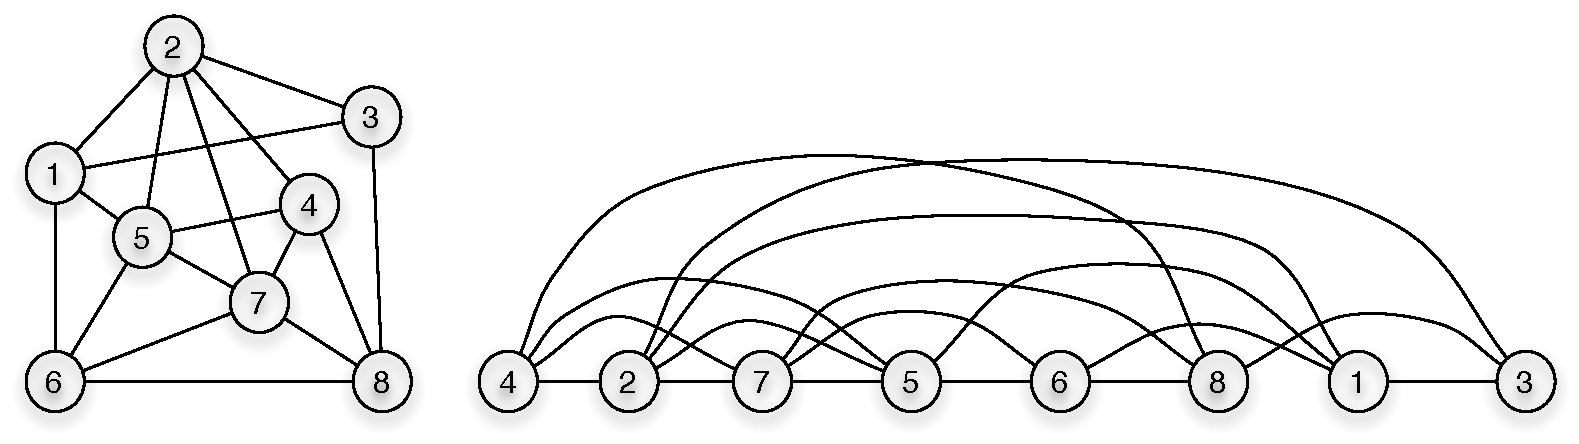
\includegraphics[width = 6in]{ordering_hw5.pdf}
	\end{center}

\noindent
(b)
Prove that the theorem in part (a) above implies the following
statement: ``If all vertices of a graph $G$ have degree at most $D$
then $G$ can be colored with at most $D+1$ colors''.
(You will cover a different proof of this theorem in the discussion. Here you
only need to show how it can be derived from part (a).)

\end{problem}

\begin{solution}
(a) Each node must have at most $k+1$ colors where $k$ is the number of neighbors among the 
verticies preceding $v_i$. 

If you have two verticies that are connected to each other, then,

\[  v_i = 1 \]
\[  k = 1 \]
\[  k + 1 = 2 \]

There are only two verticies that share an edge. They must be a distinct color, so the two verticies have a unique
color. Every time you add a new vertex, you can assume that each preceding vertex is connected to the one you add. Basically,
$v_1$ shares an edge with every vertex that is added until $v_1$. Each vertex needs a unique color, so for $v_2$ you need
$3$ colors, for $v_3$ you need $4$ colors, for $v_4$ you need $5$ colors, and so on. The trend is that you need
1 more color than the verticies that are present, so you can have at most $k+1$ colors. You can have less, but this
condition is if each preceding vertex are connected together.

(b)
Assume graph $G$ contains a vertex that has $D$ edges. Using the standards from part (a), we assume this vertex 
is $v_i$, and it has $D$ neighbors. Part (a) tells us $v_(i-1)$ has at most $D$ colors. Since $D = k$, the graph can
be colored with at most $D+1$ colors.
